%----------------------------------------------------------------------
% Homework Problem Template

\begingroup
\allowdisplaybreaks

\newpage
\section{Problem 1}

\begin{figure}[h]
	\centering
	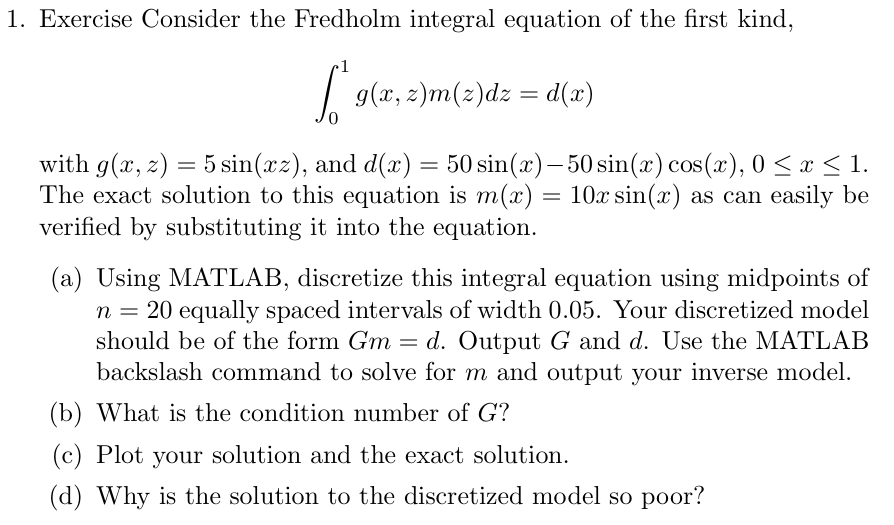
\includegraphics[width=0.8\textwidth]{./images/problem_1_statement.png}
\end{figure}

\subsection{Solution}

First, let's verify the solution of $m(x)$ via substitution. (This helped me understand the problem immensely, so I will include it here)

\begin{align*}
	\\
	\int_{0}^{1} g(x,z) m(z) dz &= d(x) \\
	\\
	\int_{0}^{1} 5 \sin(xz) m(z) dz &= 50 \sin(x) - 50 \sin(x) \cos(x) \\
	\\
	\int_{0}^{1} 5 \sin(xz) m(z) dz &= \int_{0}^{1} 5 \sin(xz) m(x) dz \\
	\\
	&= \int_{0}^{1} 5 \sin(xz) \left( 10 x \sin(x) \right) dz \\
	\\
	&= 50 x \sin(x) \int_{0}^{1} \sin(xz) dz \\
	\\
	&= - \frac{50 x \sin(x)}{x} \left[ \cos(xz) \right] |_{0}^{1} \\
	\\
	&= - \frac{50 x \sin(x)}{x} \left( \cos(x) - \cos(0) \right) \\
	\\
	&= 50 \sin(x) \left( 1 - \cos(x) \right) \\
	\\
	&= 50 \sin(x) - 50 \sin(x) \cos(x) = d(x) \,\,\,\, \textcolor{green}{\checkmark}
\end{align*}

\textcolor{red}{Put answers here}
	
\subsubsection{Part A}

\textcolor{red}{If subpart to the question exist}


